\documentclass{standalone}
\usepackage{graphicx}	
\usepackage{amssymb, amsmath, amsthm}
\usepackage{color}

\usepackage{tikz}
\usetikzlibrary{intersections, backgrounds}

\definecolor{light}{RGB}{220, 188, 188}
\definecolor{mid}{RGB}{185, 124, 124}
\definecolor{dark}{RGB}{143, 39, 39}
\definecolor{highlight}{RGB}{180, 31, 180}
\definecolor{gray10}{gray}{0.1}
\definecolor{gray20}{gray}{0.2}
\definecolor{gray30}{gray}{0.3}
\definecolor{gray40}{gray}{0.4}
\definecolor{gray60}{gray}{0.6}
\definecolor{gray70}{gray}{0.7}
\definecolor{gray80}{gray}{0.8}
\definecolor{gray90}{gray}{0.9}
\definecolor{gray60}{gray}{0.95}

\begin{document}

\begin{tikzpicture}[scale=0.35, thick]

\begin{scope}[shift={(0, 0)}]
  \draw[white] (-9, -7) rectangle (9, 7);
    
  \begin{scope}
    \clip (-7, -7) rectangle (7, 6);
        \node at (0, 0) {
\includegraphics[width=3.475cm]{gnuplot/energy_vs_funnel.eps}};
  \end{scope}
  
  \draw [->, >=stealth, line width=1] (-5 - 0.05, -5) -- +(10, 0);
  \draw [->, >=stealth, line width=1] (-5, -5 - 0.05) -- +(0, 10);
  \node[] at (0, -6) { $E$ };
  \node[] at (-9, 0) { $\log \tau$ };
\end{scope}

\begin{scope}[shift={(0, -14)}]
  \draw[white] (-9, -7) rectangle (9, 7);
    
  \begin{scope}
    \clip (-7, -7) rectangle (7, 6);
        \node at (0, 0) {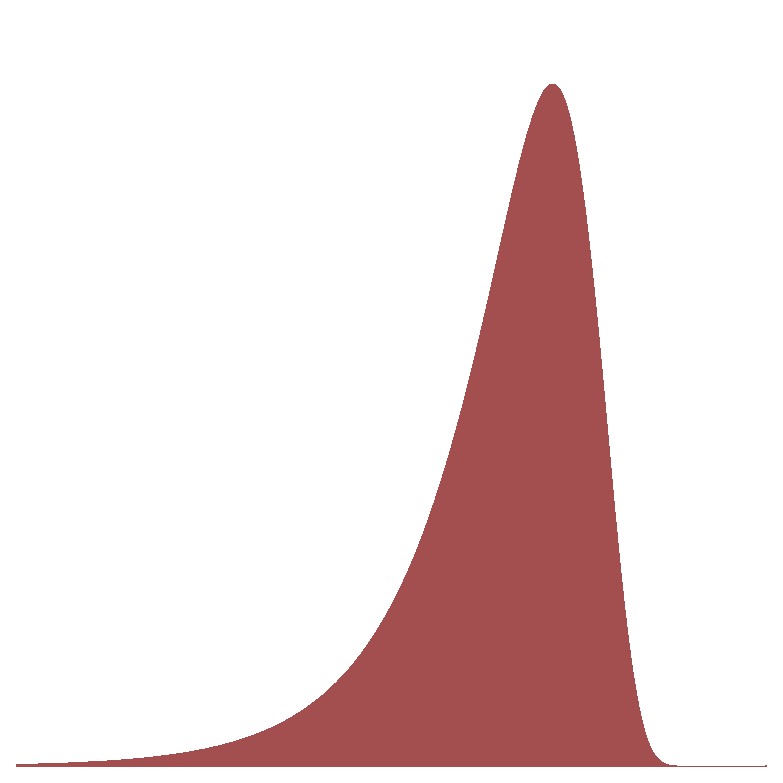
\includegraphics[width=3.475cm]{gnuplot/marginal_energy.eps}};
  \end{scope}
  
  \draw [->, >=stealth, line width=1] (-5 - 0.05, -5) -- +(10, 0);
  \draw [->, >=stealth, line width=1] (-5, -5 - 0.05) -- +(0, 10);
  \node[] at (0, -6) { $E$ };
  \node[] at (-7, 0) { $\pi(E)$ };
\end{scope}

\begin{scope}[shift={(-18, 0)}]
  \draw[white] (-9, -7) rectangle (9, 7);
    
  \begin{scope}
    \clip (-7, -7) rectangle (7, 6);
        \node at (0, 0) {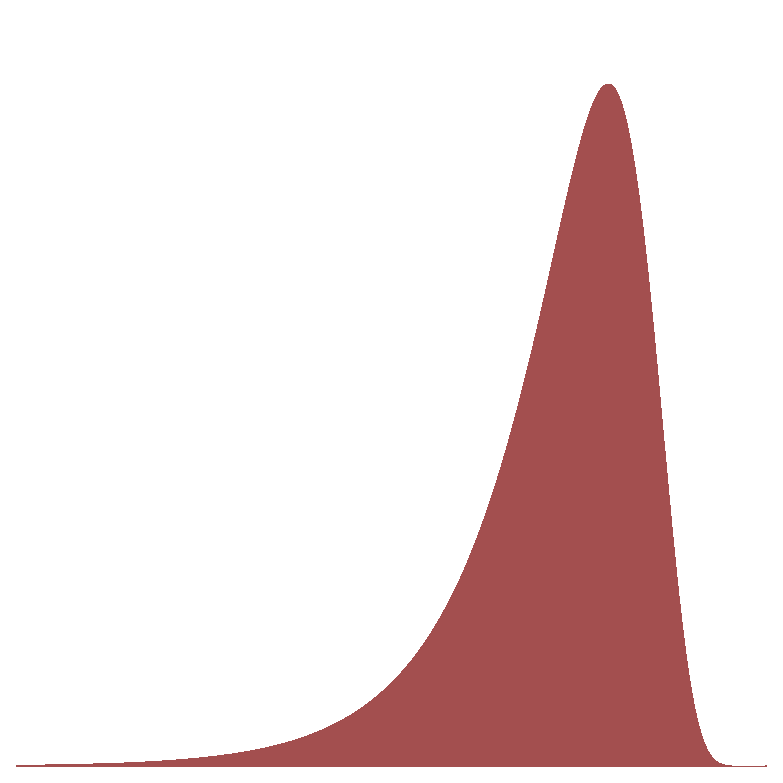
\includegraphics[width=3.475cm, angle=90]{gnuplot/log_tau.eps}};
  \end{scope}
  
  \draw [<-, >=stealth, line width=1] (-5, -5) -- +(10, 0);
  \draw [->, >=stealth, line width=1] (5, -5 - 0.05) -- +(0, 10);
  \node[] at (0, -6) { $\pi(\log \tau)$ };
\end{scope}

\end{tikzpicture}

\end{document}  